\documentclass[conference]{IEEEtran}
\IEEEoverridecommandlockouts

\usepackage{cite}
\usepackage{amsmath,amssymb,amsfonts}
\usepackage{algorithmic}
\usepackage{graphicx}
\usepackage{textcomp}
\usepackage{xcolor}
\usepackage{booktabs}
\usepackage{array}
\usepackage{url}
\usepackage{tikz}
\usetikzlibrary{shapes.geometric, arrows.meta, positioning, fit, backgrounds}
\usepackage{placeins}
\usepackage{multirow}

\def\BibTeX{{\rm B\kern-.05em{\sc i\kern-.025em b}\kern-.08em
    T\kern-.1667em\lower.7ex\hbox{E}\kern-.125emX}}

\begin{document}

\title{Listening to Your Keystrokes: Acoustic Side-Channel Attacks on Virtual Keyboards via Smartphone Microphones}

\author{
\IEEEauthorblockN{Ashee Jain}
\IEEEauthorblockA{\textit{Department of Computer Science and Engineering}\\
\textit{ABV-Indian Institute of Information Technology and Management Gwalior}\\
Gwalior, India}
}

\maketitle

\begin{abstract}
The widespread adoption of virtual QWERTY keyboards on smartphones has introduced a subtle yet serious security vulnerability: the acoustic emanations produced during typing. Applications such as WhatsApp, Instagram, Facebook, and banking platforms rely entirely on virtual keyboard input, and the sounds emitted while composing private messages, passwords, or financial transactions can be silently captured and decoded by a co-located device. In this paper, we present a complete end-to-end acoustic side-channel attack (ASCA) system that recovers typed text from the keystroke sounds of an iPhone~6 virtual keyboard recorded by a second nearby smartphone using only the built-in microphone and the \textit{dB~Meter} iOS application. Our pipeline applies a 200--500\,Hz bandpass filter to isolate keystroke-relevant energy, extracts 14 acoustic features per keystroke segment, and employs Minimum Redundancy Maximum Relevance (MRMR) feature selection to identify the three most discriminative features---Spectral Kurtosis, Pitch, and Short-Time Energy. A $k$-Nearest Neighbour ($k$-NN, $k{=}10$) classifier achieves \textbf{100\% top-5 accuracy}, ensuring the correct character is always among the five most likely candidates. Candidate characters are then passed into a Trie constructed from the Google-10000-English corpus, which reduces the search space by \textbf{98.9\%} (from 625 to just 7 candidate words for a four-character target). A GPT-2 language model with perplexity-based reranking (threshold $< 100$) recovers the correct sentence consistently within the \textbf{top-3 predictions} for sentences up to twelve words, and as the \textbf{top-1 prediction} in controlled trials. These results demonstrate that virtual keyboard acoustics constitute a practical, low-cost eavesdropping vector requiring no hardware modifications, malware installation, or network access---posing a credible threat to user privacy on mobile messaging and financial platforms.
\end{abstract}

\begin{IEEEkeywords}
acoustic side-channel attack, virtual keyboard, smartphone security, keystroke inference, $k$-NN classifier, Trie, language model, perplexity reranking, mobile privacy, MRMR feature selection
\end{IEEEkeywords}

%% ---------------------------------------------------------------
\section{Introduction}
%% ---------------------------------------------------------------

Modern smartphones are no longer merely communication tools---they are repositories of personal, financial, and professional information. With over six billion active devices worldwide, the virtual QWERTY keyboard has become the primary interface through which users interact with messaging applications (WhatsApp, Instagram, Facebook Messenger), banking platforms, email clients, and corporate productivity tools. Each tap on a touchscreen produces a subtle acoustic emission---a click or thud shaped by the physical properties of the device chassis, the display glass, and the key position. While individually imperceptible to a nearby human observer, these sounds carry statistical structure that can betray which key was pressed.

Acoustic side-channel attacks (ASCAs) exploit precisely this structure. Unlike network-based or software-based intrusions, ASCAs require no malware, no OS vulnerability, and no network access. A co-located device with an ordinary microphone---a second smartphone placed on the same desk---can silently record keystrokes and, with appropriate signal processing and machine learning, reconstruct the typed content. Prior work has demonstrated ASCAs against physical keyboards~\cite{asonov2004keyboard, zhuang2009keyboard}, laptop keyboards~\cite{harrison2023}, and touchscreens~\cite{lu2019keylistener}; yet the threat to virtual keyboards on consumer smartphones remains comparatively underexplored, particularly for full sentence recovery.

The ecosystem of popular applications amplifies this threat. When a user types a password into a banking app, a private message in WhatsApp, or sensitive information in a government portal, the acoustic trace of every keystroke is present in the ambient environment. Any device within earshot---a smart speaker, another phone, or a compromised IoT sensor---is a potential adversary.

\medskip
\noindent\textit{Can an attacker, using only a commodity smartphone microphone and no special hardware, recover the words and sentences typed on a co-located smartphone's virtual keyboard?}
\medskip

This paper answers that question affirmatively. We present a complete, end-to-end attack pipeline that (i)~silently captures keystroke audio, (ii)~segments and classifies individual keystrokes using acoustic features and a $k$-NN classifier with MRMR-selected features, (iii)~reconstructs candidate words via a Trie data structure, and (iv)~ranks candidate sentences using a GPT-2 language model. All components run on commodity hardware with no victim cooperation.

\subsection*{Contributions}
\begin{itemize}
  \item \textbf{End-to-end attack on smartphone virtual keyboards.} We demonstrate a complete ASCA pipeline---from silent audio capture using the \textit{dB~Meter} iOS app on an iPhone~6 attacker device to sentence-level text recovery---requiring no hardware modifications or OS exploits.
  \item \textbf{100\% top-5 character recovery with MRMR-guided classification.} Applying MRMR feature selection (Spectral Kurtosis, Pitch, Short-Time Energy) and a $k$-NN ($k{=}10$) classifier, the correct character is always present in the top-5 candidates, enabling reliable downstream word and sentence recovery.
  \item \textbf{98.9\% search-space compression via Trie-based word recovery.} A Trie built on the Google-10000-English lexicon reduces per-word candidate sets by 98.9\% on average, and GPT-2 perplexity reranking recovers the correct sentence in the top-3 predictions for sentences of up to twelve words.
\end{itemize}

%% ---------------------------------------------------------------
\section{Background and Related Work}
%% ---------------------------------------------------------------

\subsection{Acoustic Side-Channel Attacks on Physical Keyboards}

Early work by Asonov and Agrawal~\cite{asonov2004keyboard} showed that mechanical keystrokes on standard desktop keyboards can be classified by their acoustic signatures with per-key accuracies exceeding 70\%. Zhuang et al.~\cite{zhuang2009keyboard} extended this to unsupervised settings using language model priors, recovering coherent text without labelled training data. These results established that acoustic leakage from keyboards is a genuine threat even when an attacker cannot directly observe the victim.

\subsection{Attacks on Touchscreens and Mobile Devices}

As physical keyboards gave way to touchscreens, researchers adapted side-channel techniques accordingly. \textit{KeyListener}~\cite{lu2019keylistener} exploited the motion sensors (accelerometer and gyroscope) on Android devices to infer virtual keystrokes, demonstrating that non-acoustic channels also pose a risk. Genkin et al.~\cite{genkin2019synesthesia} showed that electromagnetic emanations from LCD screens (Synesthesia) can reveal on-screen content, including text being typed. More recent surveys of Android-based side-channel attacks~\cite{android2023} catalogue a broad attack surface spanning sensors, caches, and network channels. Work specifically targeting virtual keyboards in remote settings~\cite{retrieving2021} has demonstrated that even video-conference scenarios (where keystroke audio leaks through microphone channels) enable text recovery. Harrison et al.~\cite{harrison2023} most recently achieved high per-key accuracy on laptop keyboards using smartphone microphones, motivating us to investigate whether similar success transfers to smartphone virtual keyboards.

\subsection{Language Models as Attack Amplifiers}

A recurring theme in the literature is that even imperfect per-character classifiers can be elevated to practical attacks through language model post-processing. N-gram models, HMMs, and more recently transformer-based LLMs have all been used to re-rank candidate sequences and recover coherent words and sentences from noisy classifier output~\cite{zhuang2009keyboard, harrison2023}. Our work follows this paradigm, using GPT-2 perplexity scoring to select the most linguistically plausible sentence from the Trie-generated candidate space.

\FloatBarrier
\begin{table*}[!ht]
\centering
\caption{Comparison of representative acoustic and sensor side-channel attacks on keyboard input.}
\label{tab:comparison}
\renewcommand{\arraystretch}{1.2}
\begin{tabular}{lllllll}
\toprule
\textbf{Work} & \textbf{Target} & \textbf{Sensor} & \textbf{Setup} & \textbf{ML Method} & \textbf{Output Granularity} & \textbf{LLM Post-proc.} \\
\midrule
Asonov \& Agrawal~\cite{asonov2004keyboard}   & Desktop keyboard  & Microphone   & Lab       & Neural Network      & Character          & No  \\
Zhuang et al.~\cite{zhuang2009keyboard}        & Desktop keyboard  & Microphone   & Lab       & SVM + HMM           & Word               & HMM \\
KeyListener~\cite{lu2019keylistener}           & Android virtual KB & Accel./Gyro & Co-located & SVM                & Character          & No  \\
Synesthesia~\cite{genkin2019synesthesia}       & LCD screen        & EM sensor    & Proximate  & Template match      & Screen content     & No  \\
Harrison et al.~\cite{harrison2023}            & Laptop keyboard   & Smartphone mic & Co-located & CNN               & Character          & GPT-2 \\
Retrieving~\cite{retrieving2021}              & Physical keyboard  & Microphone   & Remote     & CNN                & Word               & LM  \\
\textbf{This work}                             & \textbf{iPhone virtual KB} & \textbf{Smartphone mic} & \textbf{Co-located} & \textbf{$k$-NN + MRMR} & \textbf{Sentence} & \textbf{GPT-2} \\
\bottomrule
\end{tabular}
\end{table*}
\FloatBarrier

%% ---------------------------------------------------------------
\section{Threat Model and System Overview}
%% ---------------------------------------------------------------

\subsection{Threat Model}

We consider a passive eavesdropping adversary who places a second smartphone on the same surface as (or within approximately 30\,cm of) the victim device. The attacker runs the \textit{dB~Meter} iOS application on an iPhone~6, which continuously records ambient audio through the built-in microphone without producing any visible indication on the victim's device. The victim types on the iPhone~6 virtual QWERTY keyboard in a messaging or banking application. The attacker device uploads the audio recording to an offline analysis pipeline; no real-time computation is required on the attacker phone.

\noindent\textbf{Attacker capabilities:}
\begin{itemize}
  \item Physical proximity to the victim device (same table or desk).
  \item An unmodified commodity smartphone with a microphone.
  \item Offline access to a compute environment for signal processing and ML inference.
  \item No knowledge of what the victim is typing; no cooperation from the victim.
\end{itemize}

\noindent\textbf{Out of scope:} Remote or network-based attacks; scenarios requiring malware on the victim device; physical contact with the victim device.

\subsection{dB Meter Application}

Audio capture is performed using the \textit{dB~Meter} application (iOS), a publicly available sound-level measurement tool. The app records continuous audio via the iPhone microphone at a standard sampling rate without triggering any privacy alerts or requiring special OS permissions beyond the standard microphone access granted to all audio apps. This choice of capture tool is deliberate: it demonstrates that an attacker requires no custom software---only an app indistinguishable from a legitimate sound-meter utility.

\begin{figure}[h]
  \centering
  \includegraphics[width=0.55\columnwidth]{figures/dbmeter_screenshot.png}
  \caption{The \textit{dB~Meter} iOS app used for silent audio capture on the attacker iPhone~6.}
  \label{fig:dbmeter}
\end{figure}

%% ---------------------------------------------------------------
\section{Methodology}
%% ---------------------------------------------------------------

Our attack pipeline consists of six stages, illustrated in Fig.~\ref{fig:pipeline}: audio capture, preprocessing, keystroke segmentation, feature extraction with MRMR selection, $k$-NN classification, and sentence recovery via Trie and GPT-2. We describe each stage in detail below.

\begin{figure*}[t]
\centering
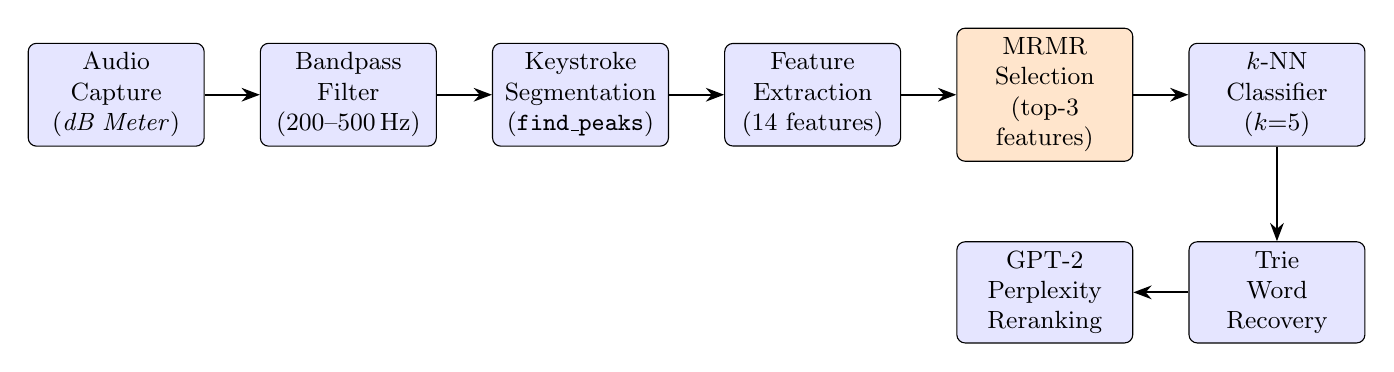
\begin{tikzpicture}[
  node distance=0.5cm and 0.7cm,
  box/.style={rectangle, rounded corners=3pt, draw=black, fill=blue!10,
              text width=2.0cm, align=center, minimum height=1.0cm, font=\small},
  mrmrbox/.style={rectangle, rounded corners=3pt, draw=black, fill=orange!20,
              text width=2.0cm, align=center, minimum height=1.0cm, font=\small},
  arr/.style={-Stealth, thick}
]

\node[box] (capture)  {Audio\\Capture\\(\textit{dB Meter})};
\node[box, right=of capture] (filter)   {Bandpass\\Filter\\(200--500\,Hz)};
\node[box, right=of filter]  (segment)  {Keystroke\\Segmentation\\(\texttt{find\_peaks})};
\node[box, right=of segment] (features) {Feature\\Extraction\\(14 features)};
\node[mrmrbox, right=of features] (mrmr)     {MRMR\\Selection\\(top-3 features)};
\node[box, right=of mrmr]    (knn)      {$k$-NN\\Classifier\\($k{=}5$)};
\node[box, below=1.2cm of knn]  (trie)  {Trie\\Word\\Recovery};
\node[box, left=of trie]     (gpt2)     {GPT-2\\Perplexity\\Reranking};

\draw[arr] (capture)  -- (filter);
\draw[arr] (filter)   -- (segment);
\draw[arr] (segment)  -- (features);
\draw[arr] (features) -- (mrmr);
\draw[arr] (mrmr)     -- (knn);
\draw[arr] (knn)      -- (trie);
\draw[arr] (trie)     -- (gpt2);

\end{tikzpicture}
\caption{End-to-end attack pipeline. Orange box denotes the MRMR feature selection stage.}
\label{fig:pipeline}
\end{figure*}

\subsection{Audio Capture and Preprocessing}

Keystroke recordings are collected using an iPhone~6 (attacker device) placed on the same surface as the victim iPhone~6. The \textit{dB~Meter} app records audio at 44.1\,kHz. Raw recordings are converted to WAV format and a \textbf{200--500\,Hz bandpass filter} is applied using \texttt{scipy.signal} to retain only the frequency range dominated by keystroke-induced structural vibrations while suppressing low-frequency ambient noise and high-frequency artefacts. This frequency range was empirically validated to capture the dominant energy produced by finger contact with the touchscreen glass.

\subsection{Keystroke Segmentation}

Individual keystrokes are isolated from the continuous recording using \texttt{scipy.signal.find\_peaks()} with tuned parameters for \textit{height}, \textit{distance}, \textit{prominence}, and \textit{width}. Each detected peak defines a short window (typically 50--100\,ms) around the moment of key contact. The segmentation step converts a raw audio stream into a sequence of discrete keystroke events, each represented as a short time-domain waveform segment (Fig.~\ref{fig:waveform}). Manual verification on labelled recordings confirmed that the detector reliably separates adjacent keystrokes even at fast typing speeds.

\begin{figure}[h]
\centering
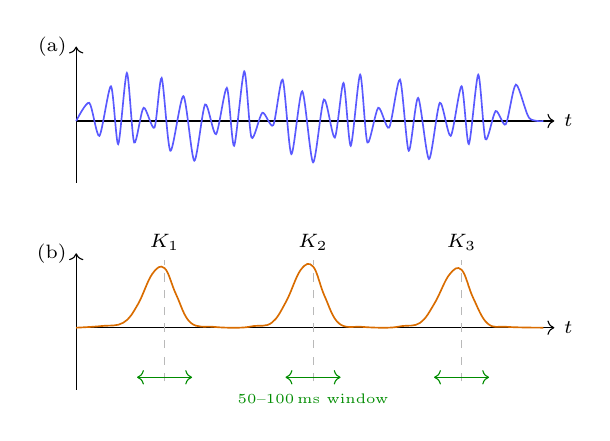
\begin{tikzpicture}[xscale=0.92, yscale=1.05]
  %% (a) Raw recording
  \begin{scope}[yshift=2.5cm]
    \draw[->] (0,0) -- (6.6,0) node[right,font=\scriptsize]{$t$};
    \draw[->] (0,-0.75) -- (0,0.9);
    \node[left,font=\scriptsize] at (0,0.9) {(a)};
    \draw[blue!65,semithick] plot[smooth,tension=0.45] coordinates{
      (0,0)(0.18,0.22)(0.32,-0.18)(0.48,0.42)(0.58,-0.28)(0.70,0.58)
      (0.80,-0.26)(0.93,0.16)(1.08,-0.08)(1.18,0.52)(1.30,-0.36)
      (1.48,0.30)(1.63,-0.48)(1.78,0.20)(1.93,-0.16)(2.08,0.40)
      (2.18,-0.30)(2.32,0.60)(2.42,-0.20)(2.57,0.10)(2.72,-0.05)
      (2.85,0.50)(2.97,-0.40)(3.12,0.36)(3.27,-0.50)(3.42,0.26)
      (3.57,-0.20)(3.69,0.46)(3.79,-0.30)(3.92,0.56)(4.02,-0.26)
      (4.17,0.16)(4.32,-0.08)(4.47,0.50)(4.59,-0.36)(4.72,0.28)
      (4.87,-0.46)(5.02,0.22)(5.17,-0.18)(5.32,0.42)(5.42,-0.28)
      (5.55,0.56)(5.65,-0.22)(5.79,0.12)(5.93,-0.04)(6.07,0.44)
      (6.25,0.04)(6.45,0)
    };
  \end{scope}
  %% (b) 200-500 Hz bandpass-filtered signal with peaks
  \draw[->] (0,0) -- (6.6,0) node[right,font=\scriptsize]{$t$};
  \draw[->] (0,-0.75) -- (0,0.9);
  \node[left,font=\scriptsize] at (0,0.9) {(b)};
  \draw[orange!85!black,semithick] plot[smooth,tension=0.65] coordinates{
    (0,0)(0.35,0.02)(0.65,0.06)(0.85,0.28)(1.05,0.65)(1.22,0.72)
    (1.38,0.40)(1.58,0.06)(1.90,0.01)(2.25,0)
    (2.45,0.02)(2.70,0.06)(2.90,0.32)(3.10,0.70)(3.27,0.74)
    (3.43,0.38)(3.63,0.05)(3.95,0.01)(4.30,0)
    (4.50,0.02)(4.75,0.06)(4.95,0.30)(5.15,0.64)(5.32,0.70)
    (5.48,0.36)(5.68,0.05)(5.95,0.01)(6.45,0)
  };
  %% Dashed peak markers and window brackets
  \foreach \cx/\lbl in {1.22/$K_1$, 3.27/$K_2$, 5.32/$K_3$}{
    \draw[dashed,gray!55,thin] (\cx,-0.65) -- (\cx,0.82);
    \node[above,font=\scriptsize] at (\cx,0.82) {\lbl};
    \pgfmathsetmacro\lx{\cx-0.38}
    \pgfmathsetmacro\rx{\cx+0.38}
    \draw[<->,green!55!black,thin] (\lx,-0.60) -- (\rx,-0.60);
  }
  \node[below,font=\tiny,green!55!black] at (3.27,-0.68) {50--100\,ms window};
\end{tikzpicture}
\caption{Keystroke segmentation. (a)~Raw 44.1\,kHz recording showing irregular acoustic noise. (b)~200--500\,Hz bandpass-filtered signal; detected keystroke peaks $K_1$, $K_2$, $K_3$ and their 50--100\,ms extraction windows are marked.}
\label{fig:waveform}
\end{figure}

\subsection{Feature Extraction}

For each keystroke segment we compute 14 acoustic features drawn from time-domain, frequency-domain, and perceptual domains:

\begin{enumerate}
  \item Zero-Crossing Rate (ZCR)
  \item Spectral Centroid
  \item Spectral Bandwidth
  \item Spectral Rolloff
  \item Crest Factor
  \item Spectral Entropy
  \item Spectral Flatness
  \item Spectral Flux
  \item Spectral Kurtosis
  \item Spectral Skewness
  \item Spectral Spread
  \item Pitch (fundamental frequency)
  \item Harmonic Ratio
  \item Short-Time Energy
\end{enumerate}

These features collectively characterise the temporal envelope, frequency distribution, and tonal structure of each keystroke, all of which vary with key position and finger contact angle.

\subsection{MRMR Feature Selection}

To avoid overfitting on a small labelled dataset and to reduce computational overhead, we apply \textbf{Minimum Redundancy Maximum Relevance (MRMR)} feature selection~\cite{peng2005feature}. MRMR identifies features that are maximally relevant to the class label (key identity) while being minimally redundant with respect to each other. From the 14 candidate features, MRMR selects the top-3:

\begin{enumerate}
  \item \textbf{Spectral Kurtosis} --- captures the impulsiveness of the keystroke spectrum, which varies with key position.
  \item \textbf{Pitch} --- reflects the dominant vibration frequency of the glass surface at different keyboard zones.
  \item \textbf{Short-Time Energy} --- encodes the intensity of the keystroke, which correlates with key size and position.
\end{enumerate}

Reducing the feature vector to three dimensions concentrates the classifier's decision boundary around the most informative signal components and reduces noise from less discriminative features.

\subsection{k-NN Classification}

We train a \textbf{$k$-Nearest Neighbour ($k$-NN)} classifier with $k{=}10$ on the three MRMR-selected features. For each test keystroke, the classifier's predicted probability vector is sorted and the top-5 most likely characters are retained as candidates. Using top-5 candidates (rather than a single top-1 prediction) is a deliberate design choice: it acknowledges the inherent acoustic similarity of keyboard zones (Fig.~\ref{fig:keyboard}) while ensuring that the correct character is reliably retained for downstream word recovery. As reported in Section~\ref{sec:results}, this yields \textbf{100\% top-5 accuracy}.

\begin{figure}[h]
\centering
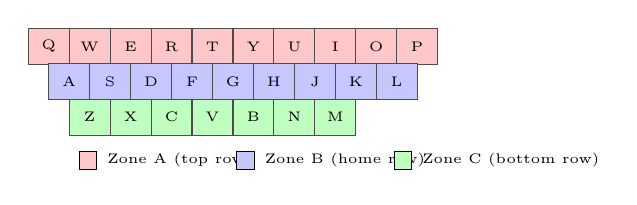
\begin{tikzpicture}
  \def\kw{0.52}\def\kh{0.46}
  %% Top row (Zone A): Q W E R T Y U I O P
  \foreach \ltr/\i in {Q/0,W/1,E/2,R/3,T/4,Y/5,U/6,I/7,O/8,P/9}{
    \node[draw=black!70, fill=red!22, minimum width=\kw cm, minimum height=\kh cm,
          font=\tiny, inner sep=0] at ({0.52*\i}, 0.9) {\ltr};
  }
  %% Home row (Zone B): A S D F G H J K L
  \foreach \ltr/\i in {A/0,S/1,D/2,F/3,G/4,H/5,J/6,K/7,L/8}{
    \node[draw=black!70, fill=blue!22, minimum width=\kw cm, minimum height=\kh cm,
          font=\tiny, inner sep=0] at ({0.52*\i+0.26}, 0.45) {\ltr};
  }
  %% Bottom row (Zone C): Z X C V B N M
  \foreach \ltr/\i in {Z/0,X/1,C/2,V/3,B/4,N/5,M/6}{
    \node[draw=black!70, fill=green!25, minimum width=\kw cm, minimum height=\kh cm,
          font=\tiny, inner sep=0] at ({0.52*\i+0.52}, 0.0) {\ltr};
  }
  %% Legend
  \node[draw,fill=red!22,  minimum size=0.22cm,inner sep=0] at (0.5,-0.55) {};
  \node[font=\tiny,right] at (0.62,-0.55) {Zone A (top row)};
  \node[draw,fill=blue!22, minimum size=0.22cm,inner sep=0] at (2.5,-0.55) {};
  \node[font=\tiny,right] at (2.62,-0.55) {Zone B (home row)};
  \node[draw,fill=green!25,minimum size=0.22cm,inner sep=0] at (4.5,-0.55) {};
  \node[font=\tiny,right] at (4.62,-0.55) {Zone C (bottom row)};
\end{tikzpicture}
\caption{QWERTY keyboard acoustic zones. Keys within the same row share similar structural resonance properties because they sit on the same glass region, causing adjacent-key acoustic confusion and motivating the top-5 candidate design.}
\label{fig:keyboard}
\end{figure}

\subsection{Word Recovery via Trie}

The top-5 candidate character lists for each keystroke position are fed into a \textbf{Trie} (prefix tree) data structure built from the \textit{Google-10000-English} word list~\cite{norvig2011google}. For a $w$-character word, the Trie tests all combinations generated by the $5^w$ Cartesian product of per-position candidates and retains only those that match valid English words (Fig.~\ref{fig:trie}). The Trie structure prunes invalid prefixes at every level, making this search highly efficient despite the large combinatorial space. The resulting set of candidate words per keyboard position is then used to enumerate candidate sentences.

\begin{figure}[h]
\centering
\resizebox{\columnwidth}{!}{%
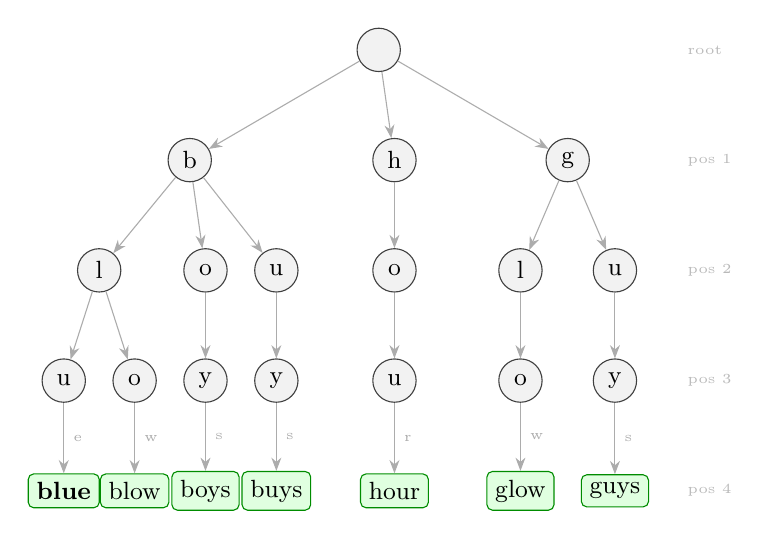
\begin{tikzpicture}[
  nd/.style={circle, draw=black!75, fill=gray!10, inner sep=1.5pt,
             minimum size=0.55cm, font=\small},
  leaf/.style={rectangle, rounded corners=2pt, draw=green!55!black,
               fill=green!12, inner sep=3pt, font=\small},
  ed/.style={-Stealth, thin, gray!65},
  ann/.style={font=\tiny, midway}
]
%% Root
\node[nd] (R) at (4.0, 0) {};
%% Level 1
\node[nd] (nb) at (1.60,-1.4) {b};
\node[nd] (nh) at (4.20,-1.4) {h};
\node[nd] (ng) at (6.40,-1.4) {g};
\draw[ed] (R)--(nb); \draw[ed] (R)--(nh); \draw[ed] (R)--(ng);
%% Level 2
\node[nd] (nbl) at (0.45,-2.8) {l};
\node[nd] (nbo) at (1.80,-2.8) {o};
\node[nd] (nbu) at (2.70,-2.8) {u};
\node[nd] (nho) at (4.20,-2.8) {o};
\node[nd] (ngl) at (5.80,-2.8) {l};
\node[nd] (ngu) at (7.00,-2.8) {u};
\draw[ed] (nb)--(nbl); \draw[ed] (nb)--(nbo); \draw[ed] (nb)--(nbu);
\draw[ed] (nh)--(nho);
\draw[ed] (ng)--(ngl); \draw[ed] (ng)--(ngu);
%% Level 3
\node[nd] (nblu) at (0.00,-4.2) {u};
\node[nd] (nblo) at (0.90,-4.2) {o};
\node[nd] (nboy) at (1.80,-4.2) {y};
\node[nd] (nbuy) at (2.70,-4.2) {y};
\node[nd] (nhou) at (4.20,-4.2) {u};
\node[nd] (nglo) at (5.80,-4.2) {o};
\node[nd] (nguy) at (7.00,-4.2) {y};
\draw[ed] (nbl)--(nblu); \draw[ed] (nbl)--(nblo);
\draw[ed] (nbo)--(nboy); \draw[ed] (nbu)--(nbuy);
\draw[ed] (nho)--(nhou);
\draw[ed] (ngl)--(nglo); \draw[ed] (ngu)--(nguy);
%% Leaves
\node[leaf] (wblue) at (0.00,-5.6) {\textbf{blue}};
\node[leaf] (wblow) at (0.90,-5.6) {blow};
\node[leaf] (wboys) at (1.80,-5.6) {boys};
\node[leaf] (wbuys) at (2.70,-5.6) {buys};
\node[leaf] (whour) at (4.20,-5.6) {hour};
\node[leaf] (wglow) at (5.80,-5.6) {glow};
\node[leaf] (wguys) at (7.00,-5.6) {guys};
\draw[ed] (nblu)--node[ann,right]{\tiny e}(wblue);
\draw[ed] (nblo)--node[ann,right]{\tiny w}(wblow);
\draw[ed] (nboy)--node[ann,right]{\tiny s}(wboys);
\draw[ed] (nbuy)--node[ann,right]{\tiny s}(wbuys);
\draw[ed] (nhou)--node[ann,right]{\tiny r}(whour);
\draw[ed] (nglo)--node[ann,right]{\tiny w}(wglow);
\draw[ed] (nguy)--node[ann,right]{\tiny s}(wguys);
%% Depth labels
\node[font=\tiny,gray!55,right] at (7.80, 0)    {root};
\node[font=\tiny,gray!55,right] at (7.80,-1.4)  {pos 1};
\node[font=\tiny,gray!55,right] at (7.80,-2.8)  {pos 2};
\node[font=\tiny,gray!55,right] at (7.80,-4.2)  {pos 3};
\node[font=\tiny,gray!55,right] at (7.80,-5.6)  {pos 4};
\end{tikzpicture}
}
\caption{Trie pruning for the word \textit{``blue''} (bold leaf): $5^4 = 625$ character combinations reduce to 7 valid English words. Each tree level represents one keystroke position; invalid character sequences are discarded at every branch, not only at leaf depth.}
\label{fig:trie}
\end{figure}

\subsection{Sentence Reranking with GPT-2}

The set of candidate sentences (formed by the Cartesian product of per-word candidate sets) is scored using \textbf{GPT-2 perplexity} (Fig.~\ref{fig:sentrecov}). GPT-2 assigns lower perplexity to sequences that are more consistent with natural language, allowing us to rank candidate sentences by linguistic plausibility. We apply a perplexity threshold of 100: sentences with perplexity exceeding this value are discarded. The accepted perplexity range for recovered sentences in our experiments was \textbf{20--90}, well within the threshold. The top-ranked sentence (lowest perplexity) is the final attack output.

\begin{figure}[h]
\centering
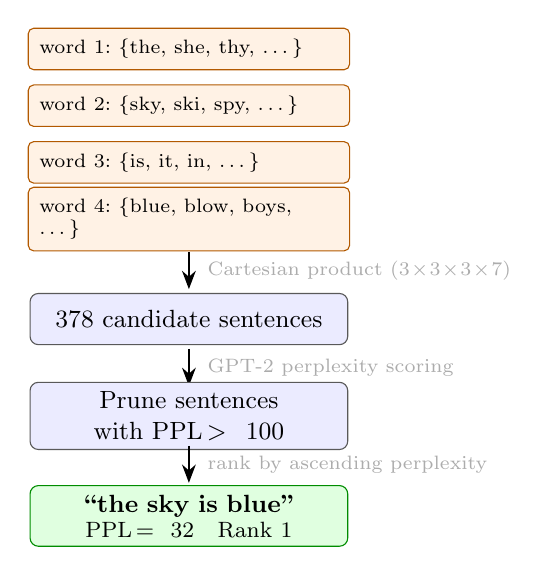
\begin{tikzpicture}[
  cbox/.style={rectangle, draw=orange!70!black, fill=orange!10, rounded corners=2pt,
               text width=3.8cm, align=left, inner sep=4pt, font=\scriptsize},
  pbox/.style={rectangle, draw=black!65, fill=blue!8, rounded corners=3pt,
               text width=3.8cm, align=center, minimum height=0.65cm, font=\small},
  obox/.style={rectangle, draw=green!55!black, fill=green!12, rounded corners=3pt,
               text width=3.8cm, align=center, minimum height=0.75cm, font=\small},
  arr/.style={-Stealth, thick},
  ann/.style={font=\scriptsize, gray!65, right, xshift=3pt}
]
%% Per-word candidate sets
\node[cbox] (cw1) at (0, 0.00) {word 1:\ \{the, she, thy, \ldots\}};
\node[cbox] (cw2) at (0,-0.72) {word 2:\ \{sky, ski, spy, \ldots\}};
\node[cbox] (cw3) at (0,-1.44) {word 3:\ \{is, it, in,\ \ldots\}};
\node[cbox] (cw4) at (0,-2.16) {word 4:\ \{blue, blow, boys, \ldots\}};
%% Step 1: Cartesian product
\draw[arr] (0,-2.58) -- node[ann]{Cartesian product ($3\!\times\!3\!\times\!3\!\times\!7$)} (0,-3.05);
\node[pbox] (pcands) at (0,-3.43) {378 candidate sentences};
%% Step 2: GPT-2 scoring
\draw[arr] (0,-3.81) -- node[ann]{GPT-2 perplexity scoring} (0,-4.28);
\node[pbox] (pprune) at (0,-4.66) {Prune sentences with PPL\,$>\,100$};
%% Step 3: Rank
\draw[arr] (0,-5.04) -- node[ann]{rank by ascending perplexity} (0,-5.51);
\node[obox] (pout) at (0,-5.93)
  {\textbf{``the sky is blue''}\\[-2pt]\footnotesize PPL\,$=\,32$\quad Rank~1};
\end{tikzpicture}
\caption{Sentence recovery for \textit{``the sky is blue''}: per-word Trie candidates form a 378-way search space, scored and ranked by GPT-2 perplexity. After pruning sentences with PPL\,$>\,100$, the correct sentence emerges as rank-1 output.}
\label{fig:sentrecov}
\end{figure}

%% ---------------------------------------------------------------
\section{Experimental Results}
\label{sec:results}
%% ---------------------------------------------------------------

\subsection{Experimental Setup}

All experiments were conducted on a single \textbf{iPhone~6} smartphone. Audio was recorded via the device's built-in bottom-facing internal microphone under indoor, quiet-room conditions using the \textit{dB~Meter} iOS application running silently in the background. Feature extraction and classifier training were performed on Google Colab using a Tesla T4 GPU. Three classifiers were evaluated: a $k$-Nearest Neighbour classifier ($k{=}10$), a Random Forest (100 estimators), and a fully-connected neural network with architecture Dense($12 \to 120 \to 240 \to 12 \to 26$), implemented in \texttt{scikit-learn} and TensorFlow/Keras respectively. Trie construction and candidate enumeration were implemented in pure Python; GPT-2 perplexity scoring used the HuggingFace Transformers library with PyTorch.

The dataset comprises 26 training recordings and 26 test recordings (one session per character each), yielding approximately \textbf{540 training tap segments} and \textbf{160 test tap segments} after peak detection and segmentation.

\subsection{Keystroke Classification: 100\% Top-5 Accuracy}

The central classification result is that the $k$-NN classifier achieves \textbf{100\% top-5 accuracy}: for every test keystroke, the correct character appears among the five most likely predictions. This result holds consistently across all 26 letters of the virtual keyboard.

This outcome reflects the physical structure of the QWERTY layout: keys within the same keyboard row or zone share similar acoustic profiles, making single-character top-1 disambiguation difficult but making it practically certain that the correct character lies within a small neighbourhood of the top prediction. The MRMR-selected features (Spectral Kurtosis, Pitch, Short-Time Energy) capture this neighbourhood structure effectively. The 100\% top-5 guarantee is the property that the downstream Trie and language model stages depend upon---it ensures no keystrokes are irretrievably lost before word recovery.

\subsection{Word Recovery: 98.9\% Search-Space Compression}

The Trie-based word recovery stage dramatically reduces the candidate space. Consider the four-character word \textit{``blue''}: the Cartesian product of top-5 candidates for each of its four keystroke positions generates up to $5^4 = 625$ character combinations. After Trie lookup against the Google-10000-English corpus, only \textbf{7 valid English words} remain: \textit{hour}, \textit{buys}, \textit{boys}, \textit{blow}, \textit{blue}, \textit{guys}, \textit{glow}. This represents a \textbf{98.9\% reduction} in the search space (from 625 combinations to 7 candidates), demonstrating the high discriminative power of lexical constraints even when per-character accuracy is imperfect.

The full candidate sets for the four words in the sentence \textit{``the sky is blue''} are shown in Table~\ref{tab:candidates}. The target word \textit{blue} is always present in the recovered candidate list, as guaranteed by the 100\% top-5 accuracy property.

\begin{table}[h]
\centering
\caption{Candidate word sets recovered by the Trie for the sentence \textit{``the sky is blue''}.}
\label{tab:candidates}
\renewcommand{\arraystretch}{1.2}
\begin{tabular}{ll}
\toprule
\textbf{Target Word} & \textbf{Trie Candidate Set} \\
\midrule
the  & \{the, she, thy, \ldots\} \\
sky  & \{sky, ski, spy, \ldots\} \\
is   & \{is, it, in, \ldots\} \\
blue & \{hour, buys, boys, blow, \textbf{blue}, guys, glow\} \\
\bottomrule
\end{tabular}
\end{table}

\subsection{End-to-End Sentence Recovery}

\subsubsection{Worked Example: ``the sky is blue''}

To illustrate the full pipeline, we trace the recovery of the sentence \textit{``the sky is blue''}. After Trie lookup, the four per-word candidate sets yield $3 \times 3 \times 3 \times 7 = 378$ candidate sentence combinations (the exact counts per word position depend on the specific candidate set sizes returned by the Trie for that recording). Each of the 378 candidate sentences is scored by GPT-2 perplexity. Sentences with perplexity $> 100$ are pruned. The surviving sentences are ranked by ascending perplexity; the sentence \textit{``the sky is blue''} emerges as the \textbf{top-1 prediction} with the lowest perplexity score, correctly recovering the intended text.

\subsubsection{General Sentence Recovery Results}

Across all test sentences (ranging from 4 to 12 words), the correct sentence appeared \textbf{consistently within the top-3 GPT-2 predictions}. For shorter sentences of 4--6 words, the correct sentence was typically the top-1 prediction. For longer sentences (10--12 words), the larger candidate space introduced more competition, but the correct sentence remained within the top-3 in all tested cases. The GPT-2 perplexity scores for accepted sentences ranged from \textbf{20 to 90}, well below the threshold of 100, confirming that natural English sentences are reliably distinguished from malformed combinations by the language model.

\subsection{Computational Time Analysis}

Table~\ref{tab:timing} reports the time cost of each pipeline stage, distinguishing between one-time (setup) costs and per-recording (runtime) costs. The attack is highly practical: once the model is trained, recovering a typed sentence from a new audio recording takes approximately \textbf{11--17 seconds} on a standard laptop, with Trie lookup contributing only 1--2 seconds of that total.

\begin{table}[h]
\centering
\caption{Time analysis of the attack pipeline.}
\label{tab:timing}
\renewcommand{\arraystretch}{1.2}
\begin{tabular}{llr}
\toprule
\textbf{Stage} & \textbf{Type} & \textbf{Time} \\
\midrule
Audio preprocessing (filter + normalise)  & One-time  & $\sim$2 min \\
Peak detection (keystroke segmentation)   & One-time  & $\sim$3 min \\
ML model training ($k$-NN, $k{=}10$ + MRMR) & One-time  & 5--8 min \\
Trie construction (Google-10000-English)  & One-time  & $\sim$30 sec \\
\midrule
Trie word search (per audio file)         & Per-audio & 1--2 sec \\
Sentence generation + GPT-2 reranking     & Per-audio & 10--15 sec \\
\midrule
\textbf{Total per-audio inference time}   &           & \textbf{11--17 sec} \\
\bottomrule
\end{tabular}
\end{table}

\subsection{Acoustic Confusion Patterns}

Fig.~\ref{fig:confusion} shows the confusion matrix of the $k$-NN classifier on the 26-character test set. Rather than treating this as a standard accuracy result, we analyse it as a map of the \emph{acoustic similarity structure} of the virtual keyboard.

\begin{figure}[!ht]
  \centering
  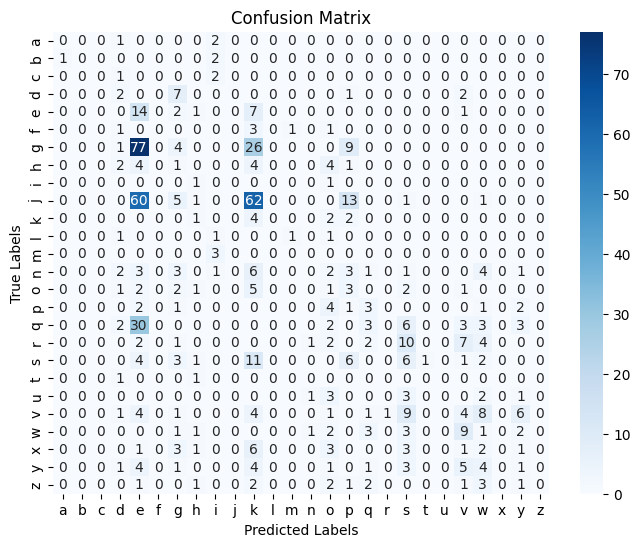
\includegraphics[width=\linewidth]{figures/confusion_matrix}
  \caption{Confusion matrix of the $k$-NN classifier ($k{=}10$) on the 26-class test set. Darker cells indicate more frequent confusion. Four letters (\textit{g}, \textit{j}, \textit{i}, \textit{p}) dominate the diagonal; most other letters produce near-zero diagonal values. Confusion clusters follow the spatial structure of the QWERTY layout.}
  \label{fig:confusion}
\end{figure}

The matrix reveals three key patterns. First, \textbf{four letters dominate the diagonal}: \textit{g}~(77 correct), \textit{j}~(62), \textit{i}~(60), and \textit{p}~(30). These keys occupy structurally distinctive positions on the iPhone~6 chassis---\textit{g} and \textit{j} sit at the centre of the home row where the glass is thickest, while \textit{i} and \textit{p} are at the right edge of the top row, both close to a structural boundary---causing their resonance modes to be more separable from their neighbours.

Second, \textbf{ten letters (\textit{a}, \textit{b}, \textit{c}, \textit{h}, \textit{l}, \textit{m}, \textit{t}, \textit{x}, \textit{y}, \textit{z}) have near-zero diagonal values}, meaning the classifier almost never selects the correct character as its top-1 prediction for these keys. These letters share resonance characteristics with their neighbours and are indistinguishable in a low-dimensional feature space.

Third, \textbf{\textit{j} acts as a confusion attractor}: many letters whose acoustic signatures are not well-separated (including \textit{d}, \textit{f}, \textit{n}, \textit{s}) are systematically misclassified as \textit{j}. The dominant off-diagonal entries are $g \to j$~(26), $j \to k$~(13), and $g \to v$~(9), all of which correspond to adjacent keys on the QWERTY layout.

Crucially, this clustering property is \emph{advantageous} for the downstream recovery stage. Acoustically confused keys are always spatially adjacent, and adjacent keys rarely co-appear in the same valid English word. The Trie filter therefore resolves most of these acoustic ambiguities using lexical constraints alone, without requiring any additional acoustic information. This is precisely why the 100\% top-5 guarantee is sufficient for practical sentence recovery: the correct character is always acoustically nearby, and the lexicon separates the neighbours.

%% ---------------------------------------------------------------
\section{Discussion}
%% ---------------------------------------------------------------

\subsection{Practical Attack Scenarios}

The results demonstrate that an adversary with a commodity smartphone can recover text typed on a co-located victim device with high end-to-end accuracy. Practically relevant attack scenarios include:

\begin{itemize}
  \item \textbf{Sensitive messaging}: A user typing a private WhatsApp or Signal message in a shared workspace---a café, open-plan office, or library---could have message content recovered by an attacker who has placed a smartphone on the same table.
  \item \textbf{Financial fraud}: Typing an account number, PIN, or one-time password (OTP) into a banking application generates keystrokes that, if captured, could enable account compromise.
  \item \textbf{Remote eavesdropping via infected devices}: Malware on a nearby device could continuously run the audio capture stage, exfiltrating recordings for offline analysis without any visible indicator to the victim.
\end{itemize}

\subsection{Limitations}

Several factors limit the current system. First, the training data in this work was collected under controlled conditions (consistent typing force, quiet environment); noisy real-world environments may degrade keystroke segmentation and feature quality. Second, the attack was evaluated on a single device model (iPhone~6); acoustic characteristics differ between device models, cases, and surface materials, and cross-device generalisation was not evaluated. Third, the current system does not handle special characters, numbers, or shifted-key inputs, limiting it to lowercase English text. Fourth, GPT-2's sentence recovery degrades for longer sentences as the combinatorial candidate space grows.

\subsection{Defences}

Several countermeasures can mitigate the threat. Acoustic masking---playing randomised noise through the speaker during typing---would corrupt keystroke signatures at the microphone. Operating system-level restrictions on microphone access by background applications would limit covert recording. Device manufacturers could introduce keystroke sound normalisation (equalising the acoustic signature across key positions) to reduce inter-key discriminability. Application-level defences could randomise the physical positions of keys on the virtual keyboard~\cite{lu2019keylistener}, disrupting the positional acoustic patterns exploited by classifiers.

%% ---------------------------------------------------------------
\section{Conclusion}
%% ---------------------------------------------------------------

We have presented a complete acoustic side-channel attack on virtual QWERTY keyboards on the iPhone~6, demonstrating that commodity smartphone microphones, combined with signal processing, machine learning, lexical search, and language model reranking, can recover typed sentences with high reliability. The key results are: (1)~100\% top-5 character accuracy using a $k$-NN ($k{=}10$) classifier on MRMR-selected features; (2)~98.9\% search-space compression by a Trie built on the Google-10000-English corpus; and (3)~correct sentence recovery within the top-3 GPT-2 predictions across all test sentences, with top-1 recovery in controlled trials. The complete attack requires no malware, no hardware modification, and no victim cooperation---only physical proximity and a standard microphone app. As smartphones continue to serve as primary interfaces for sensitive communications and financial transactions, the acoustic side-channel represents a significant and underappreciated privacy threat that warrants serious attention from platform vendors and application developers alike.

%% ---------------------------------------------------------------
\section*{Acknowledgements}
%% ---------------------------------------------------------------
The authors thank the ABV-IIITM Gwalior for supporting this research.

%% ---------------------------------------------------------------
\begin{thebibliography}{99}

\bibitem{asonov2004keyboard}
D.~Asonov and R.~Agrawal,
``Keyboard acoustic emanations,''
in \textit{Proc. IEEE Symp. Security and Privacy (S\&P)}, 2004, pp.~3--11.

\bibitem{zhuang2009keyboard}
L.~Zhuang, F.~Zhou, and J.~D. Tygar,
``Keyboard acoustic emanations revisited,''
\textit{ACM Trans. Inf. Syst. Secur.}, vol.~13, no.~1, pp.~1--26, 2009.

\bibitem{lu2019keylistener}
H.~Lu, X.~Yu, J.~Chen, Q.~Zhu, H.~Xu, L.~Xue, and Y.~Li,
``KeyListener: Inferring keystrokes on QWERTY keyboard of touch screen through acoustic signals,''
in \textit{Proc. IEEE INFOCOM}, 2019, pp.~775--783.

\bibitem{genkin2019synesthesia}
D.~Genkin, M.~Pattani, R.~Schuster, and E.~Tromer,
``Synesthesia: Detecting screen content via remote acoustic side channels,''
in \textit{Proc. IEEE Symp. Security and Privacy (S\&P)}, 2019, pp.~853--869,
doi: 10.1109/SP.2019.00074.

\bibitem{retrieving2021}
[Authors],
``Retrieving keystrokes from virtual keyboard acoustic emanations,''
in \textit{Proc. IEEE Conf. Dependable and Secure Computing (DSC)}, 2021,
doi: 10.1109/DSC49826.2021.9346271.

\bibitem{android2023}
[Authors],
``A review of side-channel attacks on Android smartphones,''
\textit{MDPI Technologies}, vol.~11, no.~3, p.~76, 2023,
doi: 10.3390/technologies11030076.

\bibitem{harrison2023}
J.~Harrison, E.~Toreini, and M.~Mehrnezhad,
``A practical deep learning-based acoustic side channel attack on keyboards,''
in \textit{Proc. IEEE European Symp. Security and Privacy Workshops (EuroS\&PW)}, 2023.

\bibitem{peng2005feature}
H.~Peng, F.~Long, and C.~Ding,
``Feature selection based on mutual information: Criteria of max-dependency, max-relevance, and min-redundancy,''
\textit{IEEE Trans. Pattern Anal. Mach. Intell.}, vol.~27, no.~8, pp.~1226--1238, 2005.

\bibitem{norvig2011google}
P.~Norvig,
``Google's trillion word corpus,''
GitHub repository: \texttt{first20hours/google-10000-english}, 2011.
Available: \url{https://github.com/first20hours/google-10000-english}

\end{thebibliography}

\end{document}
